\documentclass[tikz,border=10pt]{standalone}
\begin{document}
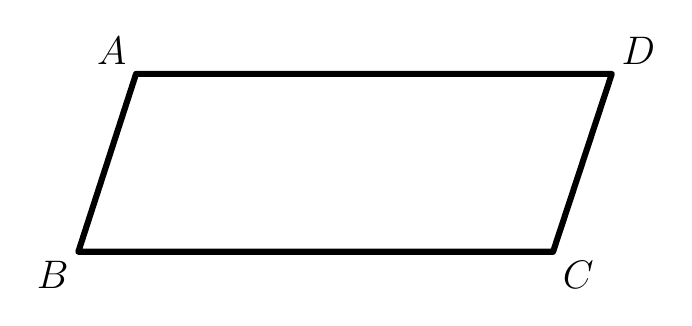
\begin{tikzpicture}
\coordinate (A) at (-2.677,1.139);
\coordinate (B) at (-3.410,-1.120);
\coordinate (C) at (2.619,-1.120);
\coordinate (D) at (3.365,1.139);



\draw[line width=2.2pt, line join=round] (A) -- (B) -- (C) -- (D) -- cycle;

\node[above left]  at (A) {\fontsize{15.5}{18.6}\selectfont $A$};
\node[above right] at (D) {\fontsize{15.5}{18.6}\selectfont $D$};
\node[below left]  at (B) {\fontsize{15.5}{18.6}\selectfont $B$};
\node[below right] at (C) {\fontsize{15.5}{18.6}\selectfont $C$};
\end{tikzpicture}
\end{document}